\documentclass[11pt,a4paper]{article}
\usepackage[margin=23mm,headheight=15pt]{geometry}
\usepackage{fontspec}
\setmainfont{Times New Roman}
\setsansfont{Arial}
\setmonofont{Consolas}[Scale=0.86]
\usepackage{amsmath,amssymb,graphicx,booktabs,tabularx,array,longtable}
\usepackage{xcolor,enumitem,fancyhdr,titlesec,hyperref,tikz}
\usetikzlibrary{arrows.meta,positioning,shapes.geometric,fit}
\definecolor{navy}{HTML}{203E65}
\definecolor{teal}{HTML}{087F8C}
\definecolor{light}{HTML}{EFF4F8}
\hypersetup{colorlinks=true,linkcolor=navy,urlcolor=teal,pdftitle={Pi Swarm - Review 2},pdfauthor={Pi Swarm Project Team}}
\setlength{\parindent}{0pt}
\setlength{\parskip}{4pt}
\setlength{\emergencystretch}{2em}
\renewcommand{\arraystretch}{1.22}
\newcolumntype{Y}{>{\raggedright\arraybackslash}X}
\setlist[itemize]{leftmargin=*,itemsep=2pt,topsep=4pt}
\setlist[enumerate]{leftmargin=*,itemsep=3pt,topsep=4pt}
\titleformat{\section}{\Large\sffamily\bfseries\color{navy}}{\thesection.}{0.6em}{}
\titleformat{\subsection}{\large\sffamily\bfseries\color{navy}}{\thesubsection}{0.6em}{}
\titleformat{\subsubsection}{\normalsize\sffamily\bfseries}{\thesubsubsection}{0.6em}{}
\pagestyle{fancy}\fancyhf{}
\fancyhead[L]{\small\sffamily PI SWARM / REVIEW 2}
\fancyhead[R]{\small\sffamily AI and Robotics}
\fancyfoot[L]{\scriptsize Amrita School of Computing, Coimbatore}
\fancyfoot[R]{\small\thepage}
\renewcommand{\headrulewidth}{0.4pt}
% Team details transcribed from the student-provided academic-details table.

\newcommand{\ProjectTitle}{Pi Swarm\\Vision-Guided Robot Navigation\\with Background Edge Computing}

\newcommand{\CourseName}{AI in Robotics --- Semester Project}

\newcommand{\GuideName}{Dr. A. Baskar}

\newcommand{\DepartmentName}{Computer Science \& Engineering}

\newcommand{\SchoolName}{Amrita School of Computing, Coimbatore}

\newcommand{\SubmissionDate}{3 November 2026}

\newcommand{\RepositoryURL}{https://github.com/Kapilkannaa/pi-swarm-robotics}

\newcommand{\TeamRows}{%

Kapil Kannaa G & CB.SC.U4CSE23036\\

Mitali Patle & CB.SC.U4CSE23038\\

Kavinraj S & CB.SC.U4CSE23329\\

Gudi Hemanth & CB.SC.U4CSE23619\\

D. Uday Kumar & CB.SC.U4CSE23655\\}


\hypersetup{pageanchor=false}
\newcommand{\citesrc}[1]{[\ref{ref:#1}]}
\newcommand{\evidence}[1]{\textcolor{teal}{\textbf{Evidence:}} #1}
\newcommand{\code}[1]{\texttt{\detokenize{#1}}}
\begin{document}
\begin{titlepage}
\begin{tikzpicture}[remember picture,overlay]
\fill[navy] (current page.north west) rectangle ([yshift=-6mm]current page.north east);
\draw[navy!15,line width=0.6pt] ([xshift=23mm,yshift=28mm]current page.south west) -- ([xshift=-23mm,yshift=28mm]current page.south east);
\end{tikzpicture}
\vspace*{5mm}
\begin{center}
{\sffamily\bfseries\color{navy}\fontsize{17}{22}\selectfont AMRITA SCHOOL OF COMPUTING}\par
\vspace{2mm}
{\sffamily\large Coimbatore}\par
\vspace{12mm}
{\sffamily\bfseries\color{teal}\Large AI and Robotics}\par
\vspace{3mm}
{\sffamily\small Case Study Report / Review 2}\par
\vspace{10mm}
{\sffamily\bfseries\color{navy}\fontsize{33}{38}\selectfont Pi Swarm\par}
\vspace{4mm}
{\sffamily\color{navy}\fontsize{20}{26}\selectfont Vision-Guided Robot Navigation\\with Background Edge Computing\par}
\vspace{5mm}\textcolor{teal}{\rule{34mm}{1.8pt}}\par
\end{center}
\vspace{5mm}
{\sffamily\bfseries\small SUBMITTED BY}\par\vspace{3mm}
\begin{tabularx}{\textwidth}{@{}X l@{}}
\toprule\textbf{Team member}&\textbf{Roll number}\\\midrule
\TeamRows\bottomrule
\end{tabularx}
\par\vspace{9mm}
\textbf{Course:} \CourseName\\[4pt]
\textbf{Guide:} \GuideName\\[4pt]
\textbf{Department:} \DepartmentName\\[4pt]
\textbf{Institution:} \SchoolName
\vfill
{\sffamily\bfseries\small PROJECT REPOSITORY}\par\vspace{2mm}
\expandafter\url\expandafter{\RepositoryURL}\par
\vspace{9mm}
\end{titlepage}
\hypersetup{pageanchor=true}
\pagenumbering{roman}
\section*{Acknowledgement}
The team thanks Dr. A. Baskar for guidance during the AI and Robotics semester
project, and the Department of Computer Science \& Engineering, Amrita School of
Computing, Coimbatore, for academic and laboratory support. The technical references
and open-source libraries used in the implementation are credited in this report
and the repository.

\section*{Abstract}
Pi Swarm uses an overhead camera to guide low-cost robots that have no onboard
navigation sensors. A laptop detects a printed marker, maps the operator's clicked
destination into floor coordinates, and sends wheel commands directly to an
ESP8266 controller. Motion is divided into short bursts so that the controller
can wait for delayed images and update its speed and turning estimates from
observed movement. A Raspberry Pi worker evaluates alternative burst settings
through Monte Carlo trajectory simulations, returning advice without blocking
the camera or motor-control loop.

The evaluation compares continuous and burst control, examines online adaptation,
and checks communication and firmware logic. In ten seeded trials with a 0.3 s
camera delay, continuous control completed none of the simulated tasks, while
burst control completed all ten. The software suite passed 181 tests. These
results describe the submitted software and simulator; historical board records
and team-reported operation are discussed separately. The work demonstrates a
practical division of vision, adaptive control, embedded actuation and background
computation for an educational robotics system.

\textbf{Keywords:} vision-guided robotics; ESP8266; Raspberry Pi; ArUco; adaptive
control; edge offloading; Monte Carlo simulation.

\section*{Evaluation scope}
This final submission includes the implementation, reproducible simulation
results and recorded bench evidence. The robots were dismantled before the final
documentation stage, so no additional physical trials or hardware video were
recorded. The accompanying demonstration video is generated from the simulator.

\clearpage\begingroup\small\setlength{\parskip}{0pt}\tableofcontents\endgroup\clearpage\pagenumbering{arabic}

\section{Introduction and Problem Definition}
\subsection{Background and Overview}
An inexpensive mobile robot can move reliably under direct commands while still
being unable to determine where it is. The available platforms consist of WEMOS
D1 Mini-class ESP8266 controllers, L298N motor drivers, and differential-drive
chassis. They contain no onboard range or position sensors. The project therefore
uses an overhead camera as an external observation source and concentrates on the
integration of vision, feedback, communication, and computation.

Two robot platforms are available to the team. The principal physical workflow is
operator-assisted click-to-go: a phone looks down at the robot, the laptop displays
the video, the operator selects a destination, and the robot moves toward that
point. The wider codebase also includes cooperative search and target convergence
in simulation. These are related evaluation capabilities, not evidence that a
two-robot physical swarm demonstration has been completed.

\subsection{Problem Statement}
The engineering problem is to guide a sensorless differential-drive robot toward
a selected floor location using delayed camera observations, while retaining
responsive stop behavior and making useful use of a Raspberry Pi. The Pi must add
compute capacity without becoming a mandatory relay between camera, controller,
and motors. A delayed background job must never delay a stop command.

\subsection{Need for the Proposed Solution}
Open-loop driving accumulates errors from wheel mismatch, floor friction, battery
condition, and uncertain command timing. Camera feedback can correct those errors,
but a controller acting continuously on old images can overshoot. A stop-and-measure
strategy is appropriate when camera latency is substantial. Background simulation
also allows alternative control settings to be examined without consuming the
laptop's time-sensitive vision/control thread.

\subsection{Objectives}
\begin{enumerate}
\item Estimate robot location from an overhead phone stream or laptop webcam.
\item Preserve the operator's click-to-go interface and direct laptop-to-robot UDP path.
\item Adapt motion estimates from observed displacement and heading changes.
\item Offload bounded trajectory-profile evaluation to a Raspberry Pi worker.
\item Enforce firmware and controller stop conditions and make failure behavior explicit.
\item Deliver source, configuration examples, test evidence, and an academic report
that another team member can reproduce.
\end{enumerate}

\subsection{Scope and Application}
The scope is a supervised indoor arena with a flat floor, controlled lighting,
and a camera covering the intended motion area. The implementation supports printed
ArUco markers and a single-robot red-LED tracking alternative. The Pi evaluates
compact state snapshots; raw camera video is not routed through it. Suitable
applications are classroom robotics demonstrations, experiments in delayed feedback,
and small-scale distributed-compute studies.

This is not an obstacle-aware production robot. There is no ultrasonic, infrared,
encoder, or onboard camera sensing. The robot must not be assumed to detect people,
furniture, drop-offs, or arbitrary obstacles. Offload estimates use assumed physics
and are advisory rather than certified safety predictions.

\subsection{Existing System and Its Limitations}
The earlier build provided laptop-side LED click-to-go and a camera-based swarm
simulator. A later integration placed the Pi in the command path. That arrangement
demonstrated real Pi computation but made Pi connectivity a prerequisite for the
new live path. The revised design restores direct laptop control and isolates the
Pi as a background worker. Table~\ref{tab:comparison} identifies the differences.

\begin{table}[ht]\centering\small
\begin{tabularx}{\textwidth}{@{}lYYY@{}}\toprule
Property & Open-loop commands & Earlier Pi coordinator & Revised project\\\midrule
Feedback & None & External camera & External camera\\
Motor sender & Laptop/tool & Pi & Laptop\\
Pi contribution & None & Inference and control & Background rollouts\\
Pi unavailable & Not applicable & Command path interrupted & Local control remains available\\
Main limitation & Accumulated drift & Extra critical dependency & External vision and assumed models\\\bottomrule
\end{tabularx}
\caption{Architectural comparison. Availability does not imply safe motion without a fresh camera observation.}\label{tab:comparison}
\end{table}

\clearpage\section{Proposed System and Design}
\subsection{Proposed Solution}
The laptop is responsible for decoding the phone stream, estimating robot pose,
accepting a click, and generating motion commands. Its controller advances in short
bursts and waits for delayed imagery to catch up. The Pi independently evaluates
three candidate burst profiles under randomized speed, wheel gain, camera delay,
and packet-loss assumptions. The laptop displays and logs the returned comparison.
It does not automatically apply the recommendation to moving hardware.

The offload client keeps only the newest requested goal. It rejects a result that
belongs to a cancelled or superseded goal. If authentication fails, the Pi is busy,
or a connection times out, the worker state becomes unavailable while local
camera/control continues. This separation is the central design decision.

\subsection{System Requirements}
\subsubsection*{Hardware requirements}
\begin{tabularx}{\textwidth}{@{}lY@{}}\toprule
Component & Role and constraints\\\midrule
Two ESP8266 robot platforms & D1 Mini-class controller, L298N, two drive motors and caster. Each uses its own firmware ID and direction flags.\\
Raspberry Pi Zero W & Background compute worker, using standard-library Python. It is not expected to outperform a modern laptop.\\
Phone or laptop camera & External visual sensing; overhead orientation and sufficient marker/LED visibility are required.\\
Laptop & Vision processing, interface, adaptive control, and direct UDP sender.\\
Wi-Fi network & Common 2.4 GHz network with device-to-device traffic. ESP8266 is a 2.4 GHz device \citesrc{esp}.\\
Power system & Robot battery supply and correctly isolated USB/5 V arrangements; physical setup must be checked by the team.\\\bottomrule
\end{tabularx}

\subsubsection*{Software requirements}
Python 3.12 is the reference laptop environment. The camera path uses OpenCV,
NumPy and Pillow; pytest validates software behavior. The Pi worker needs Python
3.11 or later and no OpenCV installation. Arduino CLI with the ESP8266 core builds
firmware. C++ host tests exercise the same parser and safety logic used by the sketch.
The public repository includes pinned laptop dependencies and example configuration.

\subsection{System Architecture}
Two separate data paths are used. The control path is
\textit{camera $\rightarrow$ laptop $\rightarrow$ ESP8266}. The compute path is
\textit{laptop snapshot $\rightarrow$ Pi worker $\rightarrow$ laptop advice}.
Both use Wi-Fi, but they have different timing requirements. Only the first path
determines immediate robot actuation. The offload server never opens a robot UDP socket.

Each robot is addressed using its firmware ID and network endpoint. A printed
marker's ID is a vision identity, not proof of that firmware ID. The team-provided
marker photograph decoded as ArUco ID 1; if that marker is fitted to firmware bot 2,
the runner must explicitly use \code{--bot 2 --marker-id 1}. Two visible robots
must have distinct marker identities.

\subsection{Block Diagram}
\begin{figure}[ht]\centering
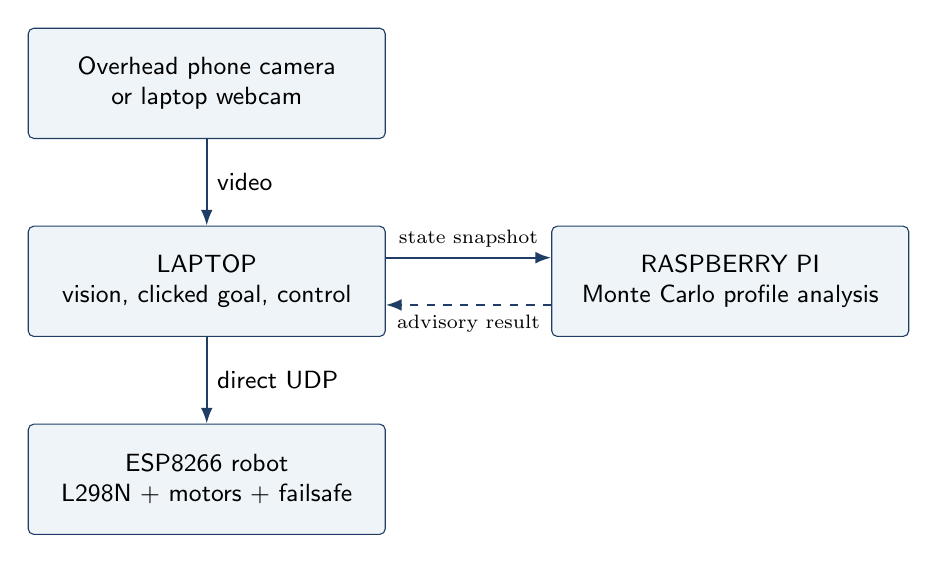
\begin{tikzpicture}[font=\small\sffamily,node distance=11mm,
box/.style={draw=navy,rounded corners=2pt,fill=light,align=center,text width=43mm,minimum height=14mm},
arr/.style={-{Latex[length=2mm]},thick,draw=navy}]
\node[box] (cam) {Overhead phone camera\\or laptop webcam};
\node[box,below=of cam] (pc) {LAPTOP\\vision, clicked goal, control};
\node[box,below=of pc] (bot) {ESP8266 robot\\L298N + motors + failsafe};
\node[box,right=21mm of pc] (pi) {RASPBERRY PI\\Monte Carlo profile analysis};
\draw[arr] (cam)--node[right]{video}(pc);
\draw[arr] (pc)--node[right]{direct UDP}(bot);
\draw[arr] ([yshift=3mm]pc.east)--node[above,font=\scriptsize]{state snapshot}([yshift=3mm]pi.west);
\draw[arr,dashed] ([yshift=-3mm]pi.west)--node[below,font=\scriptsize]{advisory result}([yshift=-3mm]pc.east);
\end{tikzpicture}
\caption{Current architecture. The Pi compute branch is outside the motor-command path.}
\end{figure}

\subsection{System Workflow}
\begin{enumerate}
\item Configure the measured arena size, camera source, robot endpoint and identity mapping.
\item Calibrate image-to-floor coordinates from four ordered floor-corner clicks.
\item Detect the selected ArUco marker, or the configured LED in the single-robot mode.
\item Convert an operator click to a bounded floor goal; estimate motion locally.
\item Send bounded commands directly from laptop to robot, while checking vision freshness.
\item Submit an optional compact goal snapshot to the Pi on a background thread.
\item Display the Pi comparison when it matches the current job; discard obsolete advice.
\item Stop on operator request, tracking failure, stale imagery, or process exit.
\end{enumerate}

\subsection{Functional and Non-Functional Requirements}
\begin{tabularx}{\textwidth}{@{}lYY@{}}\toprule
Type & Requirement & Verification\\\midrule
Functional & Click-to-go and stop controls & Closed-loop synthetic-camera tests; physical team demonstration\\
Functional & Marker and robot ID separated & Marker tests and explicit CLI arguments\\
Functional & Pi profile-comparison job & Deterministic rollout test and HTTP worker interface\\
Safety & No background job may issue motor commands & Module separation; result marked advisory\\
Safety & Reject stale/invalid observations & Controller/firmware regression tests\\
Performance & Background HTTP must not block control & Nonblocking client and offline-worker test\\
Reproducibility & Source, seeds and result files retained & Evidence manifests and build instructions\\
Security & Credentials absent from publication & Allowlist staging and secret scan before publishing\\\bottomrule
\end{tabularx}

\clearpage\section{AI and Robotics Methodology}
\subsection{AI/ML Technique and Algorithm}
The primary adaptive element is online system identification. The controller
estimates how fast the robot travels and turns from the observed effect of its
previous burst. This differs from a fixed lookup table: observations update the
parameters that size the next burst. A heading-error integrator or burst drift
estimate compensates left/right mismatch. LED tracking additionally infers heading
from displacement, because one bright dot does not directly encode orientation.

The Pi's contribution is model-based evaluation. It simulates candidate burst
profiles under uncertain dynamics and reports empirical completion counts, travel
time and boundary proximity. This is a planning/analysis technique, not a learned
neural network. A separate supervised red-round-token classifier exists in the
earlier camera-to-Pi indicator demo. That optional demonstration is not necessary
for manually selected click-to-go goals and is not represented as the navigation
controller's perception model.

\subsection{Dataset / Input Data}
The runtime inputs are camera frames, a four-point floor calibration, robot
identity, an operator-selected pixel location, and configuration values. ArUco
markers are coded fiducials from OpenCV's \code{DICT_4X4_50}, rather than a dataset
on which this team trained a visual recognizer \citesrc{opencv}. The LED alternative
uses brightness, redness, blob area and proximity constraints.

Evaluation has three distinct input sets: seeded simulator conditions; historical
firmware/communication bench records; and teammate-reported phone-camera operation.
Only the first set supports the statistical comparisons in this report. The
optional classifier was trained on 1,200 generated examples and evaluated on 400
separately seeded examples. Its stored 400/400 result is a synthetic-data result;
real-room generalization has not been established.

\subsection{Data Preprocessing and Model Development}
\subsubsection*{Geometric calibration and pose}
Four clicked arena corners define a planar homography. Pixel location $(u,v)$ and
floor coordinates $(x,y)$ satisfy
\begin{equation}
\lambda\begin{bmatrix}x\\y\\1\end{bmatrix}
=H\begin{bmatrix}u\\v\\1\end{bmatrix}.
\end{equation}
Corners are ordered bottom-left, bottom-right, top-right and top-left. The code
rejects non-finite or degenerate quadrilaterals and incompatible saved arena
dimensions. Homography corrects projective geometry for a plane; it does not remove
camera lens distortion or the height error of a marker above the floor.

For a marker, transformed corners define its centre and a front vector from centre
to its top edge. Heading is $\theta=\operatorname{atan2}(f_y,f_x)$. The marker should
be flat, near the robot centre, with its top edge facing the physical front. ArUco
dictionary design and orientation recovery are described in the original literature
and OpenCV documentation \citesrc{aruco}\citesrc{opencv}.

\subsubsection*{Differential-drive formulation}
Let $v_L,v_R$ be wheel linear velocities and $b$ the wheel separation. The standard
planar approximation is \citesrc{robotics}
\begin{align}
v&=\frac{v_R+v_L}{2}, & \omega&=\frac{v_R-v_L}{b},\\
\dot{x}&=v\cos\theta, & \dot{y}&=v\sin\theta, & \dot{\theta}&=\omega.
\end{align}
The simulator applies a midpoint-heading integration, wheel-gain variation,
stiction, transport delay and packet loss. Reference simulator values such as
$b=0.10$ m and nominal wheel speed $0.20$ m/s are model assumptions, not measured
dimensions or speeds of the team robots.

\subsubsection*{Goal error and burst sizing}
For a goal $g=(x_g,y_g)$, distance and wrapped heading errors are
\begin{align}
d&=\sqrt{(x_g-x)^2+(y_g-y)^2},\\
e_\theta&=\operatorname{wrap}\big(\operatorname{atan2}(y_g-y,x_g-x)-\theta\big).
\end{align}
The burst controller first rotates when angular error is large, then advances.
With undershoot factor $\eta$ and estimated motion rates $\hat{v},\hat{\omega}$,
the intended burst durations are bounded versions of
\begin{equation}
\tau_{\rm turn}=\eta\frac{|e_\theta|}{\max(\hat\omega,\epsilon_\omega)},
\qquad \tau_{\rm forward}=\eta\frac{d}{\max(\hat v,\epsilon_v)}.
\end{equation}
After a burst, the robot is commanded to stop. The controller waits for configured
camera delay plus a settling margin before learning from the new observation.
This sacrifices speed to avoid repeatedly steering on an old pose.

\subsubsection*{Online adaptation}
For commanded burst duration $\Delta t_b$, observed forward displacement $\Delta s$
and signed turn progress $\Delta\theta$, smoothed estimates follow
\begin{align}
\hat v_{k+1}&=(1-\alpha)\hat v_k+\alpha\frac{\Delta s}{\Delta t_b},\\
\hat\omega_{k+1}&=(1-\alpha)\hat\omega_k+\alpha\frac{|\Delta\theta|}{\Delta t_b}.
\end{align}
The implementation uses bounded estimates and a smoothing weight of $0.5$ for
these rate updates. Little measured movement triggers an increase in burst power,
up to a command ceiling. Drift trim is also bounded. These mechanisms are useful
only when the pose measurement is credible; they do not make a lost marker safe
to ignore.

\subsection{Robotics Components}
\subsubsection*{Sensors}
The overhead camera is the only navigation sensing source. ArUco provides both
position and heading; one LED provides position and requires motion-based heading
inference. No onboard proximity or odometry sensors are fitted. The term
``sensorless robot'' refers to the onboard build, not to a system with no sensing.

\subsubsection*{Actuators}
Two geared DC motors form the differential drive. The L298N switches motor
direction and PWM inputs. The marker output currently uses the D1 Mini's onboard
LED as a demonstrator; no installed laser is claimed. The signed command range is
$[-100,100]$ and the firmware caps PWM duty at 72\%. Duty limiting is not a
substitute for checking supply voltage, driver losses and motor ratings.

\subsubsection*{Controller}
The laptop contains the adaptive motion controller. The ESP8266 is an actuator
endpoint with independent safety logic. Fixed motor inputs use D1, D2, D5 and D6;
robot-specific swap/inversion flags account for physical wiring. D3/D4/D8 are not
used for external motor wiring. The onboard LED is handled only after boot.

\subsection{AI and Robotics Integration}
The proposed integration is deliberately asynchronous. When a new click produces
a usable pose/goal pair, the laptop submits arena dimensions, pose, goal and
control assumptions to \code{/evaluate}. The default job runs 12 seeded trials
for each of three profiles. At most one job executes on the Pi, and the laptop
keeps only its newest pending goal. Results contain the job ID and goal, which
must match before the UI accepts them.

The returned recommendation compares simulated completion, boundary proximity and
mean time. It is displayed and logged, but it does not alter the active motor
controller. This preserves the previously working local workflow and prevents
unverified model assumptions from becoming automatic hardware commands. Pi Zero W
offloading here means moving work away from the control thread, not claiming an
overall speedup over the laptop.

\subsection{Algorithm and Flowchart}
\begin{figure}[ht]\centering
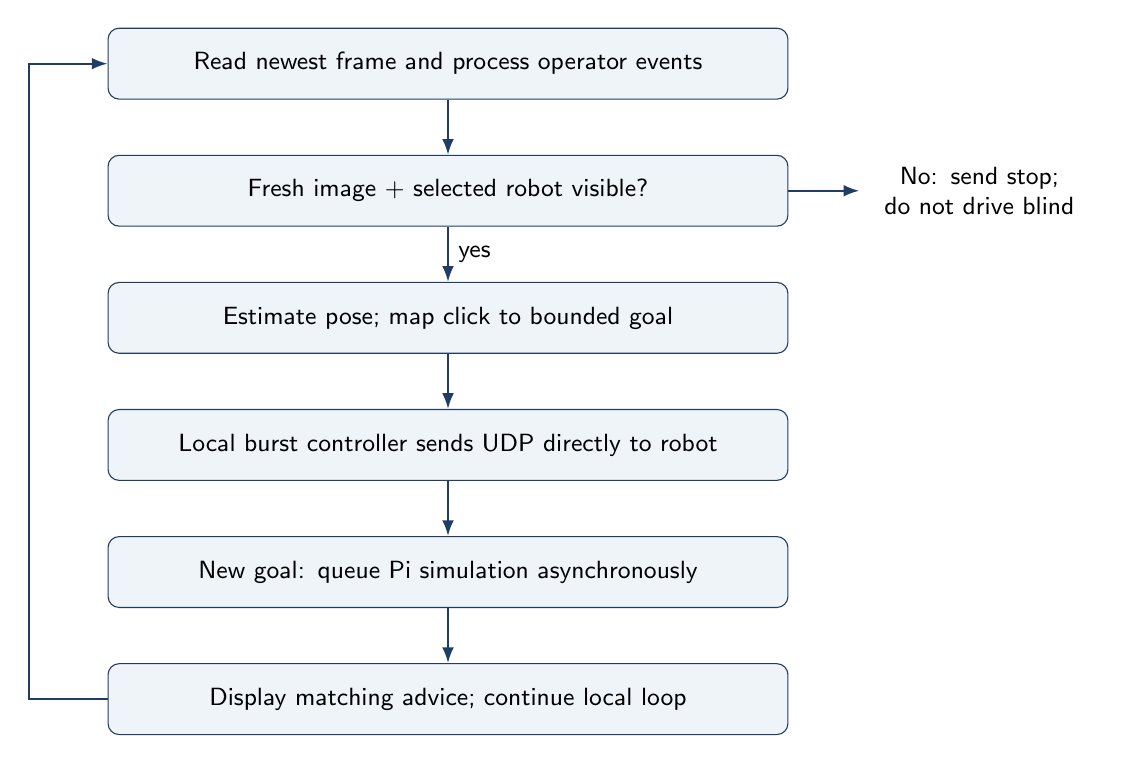
\begin{tikzpicture}[font=\small\sffamily,node distance=7mm,
process/.style={draw=navy,rounded corners,fill=light,align=center,text width=84mm,minimum height=9mm},
arr/.style={-{Latex[length=2mm]},draw=navy,thick}]
\node[process] (a) {Read newest frame and process operator events};
\node[process,below=of a] (b) {Fresh image + selected robot visible?};
\node[process,below=of b] (c) {Estimate pose; map click to bounded goal};
\node[process,below=of c] (d) {Local burst controller sends UDP directly to robot};
\node[process,below=of d] (e) {New goal: queue Pi simulation asynchronously};
\node[process,below=of e] (f) {Display matching advice; continue local loop};
\draw[arr] (a)--(b);\draw[arr] (b)--node[right]{yes}(c);\draw[arr] (c)--(d);\draw[arr] (d)--(e);\draw[arr] (e)--(f);
\draw[arr] (f.west)--++(-10mm,0)|-(a.west);
\node[align=center,right=9mm of b,text width=28mm] (stop) {No: send stop;\\do not drive blind};
\draw[arr] (b.east)--(stop.west);
\end{tikzpicture}
\caption{Control and offload workflow. Operator stop and stale-vision handling remain local.}
\end{figure}

\clearpage\section{Implementation, Testing and Results}
\subsection{Hardware Implementation}
The team assembled two Wi-Fi robot platforms. Earlier chip/upload records identify
an ESP8266EX with 4 MB flash on the tested platform. Recorded motor orientation
settings differ between firmware bot 1 and bot 2. These must not be overwritten
simply because a printed marker has a different ID.

The supplied hardware bench record documents 10 accepted zero-speed commands,
reported marker-on state, marker-off state after a continued three-second request
stream, successful re-arm, and marker-off state after 650 ms without a command.
It also records a motor lock and final outputs of zero. This validates reported
firmware states and communication, not wheel direction, physical braking distance
or a completed navigation trial. The user separately reports a teammate's successful
phone-camera click-to-go run; no numerical arrival-error series accompanies it.

\subsection{Software Implementation}
\begin{tabularx}{\textwidth}{@{}lY@{}}\toprule
Module / entry point & Responsibility\\\midrule
\code{scripts/click_go.py} & Camera UI, click events, direct robot sender; LED and ArUco modes; optional background offload.\\
\code{swarm/marker_go.py} & Marker-based pose-to-goal control and immediate stop when the selected marker is missing.\\
\code{swarm/click_control.py} & Position-only LED heading inference and adaptive burst behavior.\\
\code{swarm/control.py} & Continuous and burst controllers with online identification.\\
\code{swarm/offload_client.py} & Nonblocking latest-goal job submission and stale-result rejection.\\
\code{swarm/offload_server.py} & Authenticated, bounded background worker; no robot transport.\\
\code{swarm/offload.py} & Seed-matched Monte Carlo profile comparison.\\
\code{firmware/bot/logic.h} & Strict parser, watchdog, PWM and marker safety rules.\\\bottomrule
\end{tabularx}

The old Pi-central coordinator and indicator demo are retained as historical
experiments, not the default Review 2 control path. The offload installer stops
the previous Pi command-sending service before enabling the compute-only worker,
preventing competing senders from interfering with the laptop.

\subsection{Working Model / Prototype}
The physical prototype demonstrates a sensorless actuator node connected to a
camera-guided laptop. The reviewed software now includes explicit printed-marker
tracking for the pictured marker as well as the older LED mode. The teammate's
reported top-down phone workflow is preserved in the operator interface. The Pi
offload worker is a software implementation; the fresh offload measurements below
were executed on the laptop. No physical-Pi runtime is reported in this submission.

\subsection{Testing and Validation}
Validation is layered so that a simulator cannot silently stand in for physical
results. Unit tests cover geometry, parsing, adaptation and cancellation. A C++
harness compares firmware safety logic against the Python model. Synthetic-camera
tests render markers/LEDs and recover their geometry. Loopback tests exercise
video, HTTP and UDP transport without moving a robot. New tests cover offline
offload nonblocking behavior, cancellation, invalid jobs, and marker identity.

The fresh complete run on 3 November 2026 passed \textbf{181 tests} in 243.58 seconds. This includes firmware-model comparisons, vision geometry, controller behavior, loopback transport, marker tracking, and background-offload regression checks. The complete output is retained in \code{evidence/test_results.txt}. These are software results, not physical navigation trials.



\begin{table}[ht]\centering\small
\begin{tabularx}{\textwidth}{@{}lYY@{}}\toprule
Evidence level & Available evidence & What it does not prove\\\midrule
Software tests & Fresh automated results and saved test log & Mechanical/electrical correctness\\
Simulation & Seeded controller and offload comparisons & Real-room success probability\\
Historical hardware bench & Command counters and reported output/indicator states & Navigation accuracy or stopping distance\\
Teammate report & Successful overhead phone click-to-go described by the user & A measured multi-trial performance distribution\\
Unmeasured hardware properties & Calibration error, arrival error, latency and floor trials & Outside the recorded evaluation\\\bottomrule
\end{tabularx}
\caption{Evidence classification used throughout this report.}
\end{table}

\subsection{Performance Evaluation}
The normal scenario is a two-robot search/converge/mark simulation in a 1.00 m by
0.75 m arena. This inherited task is used to compare the shared controllers;
it is not a measurement of the manually clicked physical workflow. Each row in
Table~\ref{tab:scenarios} contains 10 seeded trials. Success means the simulator's
marker ray satisfied its target criterion. ``Contacts'' counts simulated robot
contact events. A dash means no successful trial supplied a time statistic.

\begin{table}[ht]\centering\small

\begin{tabularx}{\textwidth}{@{}Yrrrr@{}}\toprule

Scenario & Success & Mean (s) & Worst (s) & Contacts\\\midrule

Fast camera / continuous & 10/10 & 15.21 & 50.30 & 0\\

Delayed camera / continuous & 0/10 & -- & -- & 0\\

Delayed camera / burst & 10/10 & 34.39 & 49.85 & 0\\

Burst + 15\% packet loss & 10/10 & 32.84 & 53.70 & 0\\

Burst + 25\% wheel mismatch & 10/10 & 36.93 & 66.40 & 0\\

\bottomrule\end{tabularx}

\caption{Fresh simulation scenarios, 10 seeds per row, generated 3 November 2026. These are not physical robot results.}\label{tab:scenarios}\end{table}

The fresh learning ablation drives a single simulated robot through three
waypoints with a weak wheel, stiction and camera lag. With poor initial rate
estimates, online learning completed 10/10 courses; disabling learning completed
0/10. With correct initial estimates and learning disabled, 10/10 completed in a
slightly shorter mean time. Table~\ref{tab:ablation} therefore demonstrates the
value and cost of adaptation, rather than asserting that learning is always faster.

\begin{table}[ht]\centering\small

\begin{tabularx}{\textwidth}{@{}Yrr@{}}\toprule

Variant & Completed & Mean time (s)\\\midrule

learning ON,  poor initial guesses & 10/10 & 52.08\\

learning OFF, correct initial guesses & 10/10 & 49.49\\

learning OFF, poor initial guesses & 0/10 & --\\

\bottomrule\end{tabularx}

\caption{Fresh learning ablation. Mean time is computed only for completed courses.}\label{tab:ablation}\end{table}

A separate synthetic-camera click-to-go run used printed marker ID 1 with firmware bot ID 2 and the goal $(0.75,0.50)$ m. It ended at approximately $(0.73,0.50)$ m with a rounded final error of 16 mm. This tests the new marker identity mapping and local goal controller in simulation; it is not a measured physical arrival error. The console result is retained in \code{evidence/marker_click_demo.txt}.
The recorded video uses a separate seed-7 run with delayed observations and a
one-second marker occlusion. It reaches the same goal in 17.45 simulated seconds
with a true final error of 20.7 mm; its per-step log is stored under \code{media/}.

For the new background job, a clicked goal at $(0.80,0.55)$ m from pose
$(0.20,0.20,0)$ was evaluated using 12 trials per profile. All three profiles
completed 12/12 simulations. Conservative, current and longer-burst mean simulated
times were 18.78, 16.05 and 15.21 s, respectively. The job executed 12,009 integration
steps. Its measured compute time is stored with the result file; the execution
host is explicitly the laptop, not the Pi. The recommendation was not applied to
the physical motors.

\subsection{Results and Discussion}
The main observation is the difference between low-latency and delayed feedback.
Continuous control succeeds in the fresh low-lag reference trials but fails all
10 trials in the 0.3 s delayed-camera comparison. Burst control succeeds in all
10 under the same nominal delay, with longer completion times because it waits
between actions. The packet-loss and wheel-mismatch variants also succeed in this
small seeded sample. Their differing mean times should not be ranked as precise
physical performance: randomized paths, arrival thresholds and finite sample size
affect the comparison.

The offload integration meets its architectural objective: the laptop can continue
while the worker is unavailable, and a cancelled goal cannot receive an obsolete
result. This supports reliability of the software split. It does not establish
that Raspberry Pi execution is faster or that advisory profiles are safe on
unmeasured hardware. Physical calibration and Pi timing are outside the recorded evaluation.

Configuration checks, fresh observations and a single motor-command sender reduce
ambiguity when communication is intermittent. Private network settings are excluded
from the public source.

\subsection{Screenshots / Prototype Photographs}
Figure~\ref{fig:synthetic} is a frame from the simulation video. The recording
shows a selected goal, marker-based movement, a lost-marker stop command and a
background worker response. Its tracker, controller and HTTP worker are executed
on the laptop. The video, trajectory and worker output are included under
\code{media/}; no physical robot footage or Pi runtime is represented.

\begin{figure}[!htbp]\centering
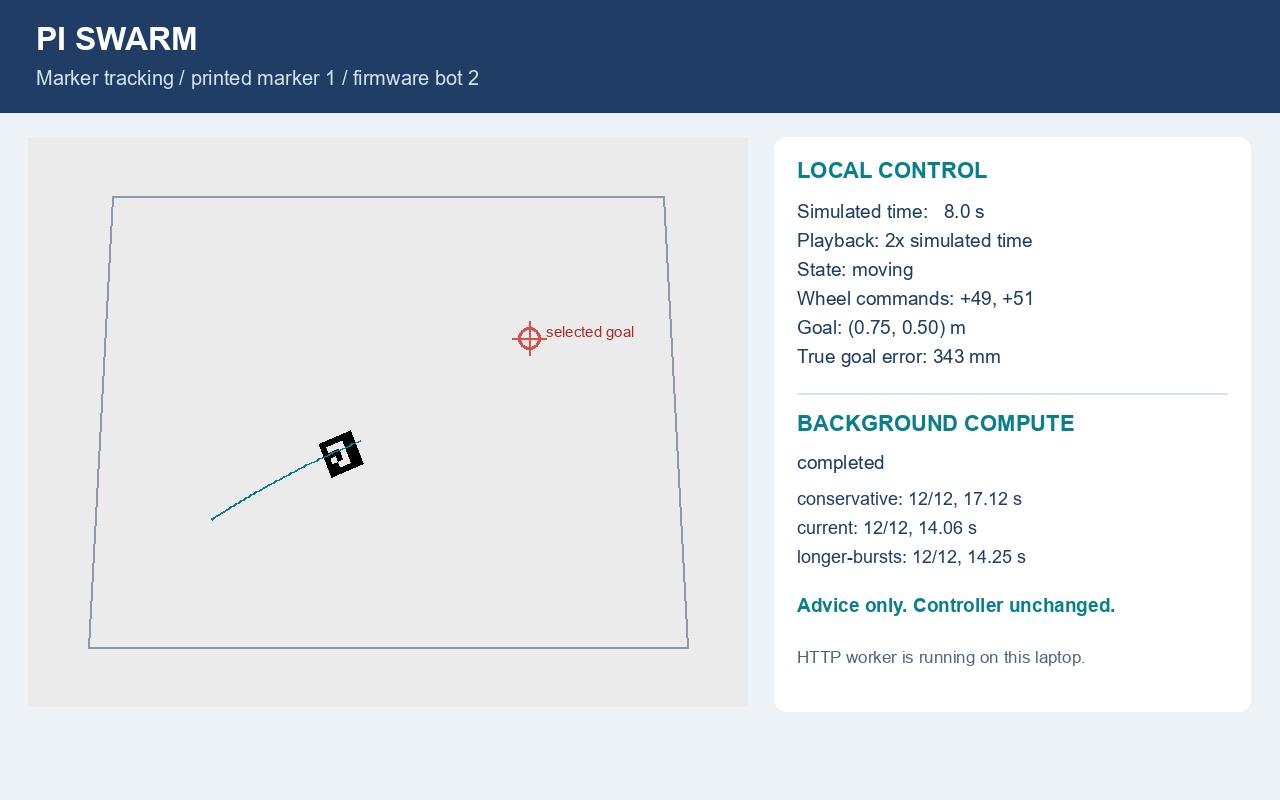
\includegraphics[width=.6\textwidth]{figures/simulation_demo.png}
\caption{Frame from the recorded software demonstration. A generated marker image
feeds the local controller while an actual local HTTP worker returns profile
comparisons. The image does not depict physical robot operation.}\label{fig:synthetic}
\end{figure}

\clearpage\section{Conclusion and Future Scope}
\subsection{Summary of the Work}
Pi Swarm combines external visual sensing, adaptive local control and distributed
background computation using low-cost robot hardware. The final architecture
preserves the established phone-camera click-to-go workflow and moves optional
simulation work to the Pi without relaying motor commands through it. The repository
provides firmware, camera/control code, the compute worker, tests, evidence and a
rebuildable LaTeX report.

\subsection{Achievement of Objectives}
\begin{tabularx}{\textwidth}{@{}YY@{}}\toprule
Objective & Assessment\\\midrule
Visual robot localization & Marker and LED geometry tested synthetically; live calibration accuracy was not measured.\\
Direct click-to-go control & Local interface preserved; teammate-reported physical operation; no quantitative physical trial series recorded.\\
Adaptive behavior & Rate/trim learning implemented and ablation-tested in simulation.\\
Useful Pi offloading & Asynchronous profile evaluation implemented; laptop validation complete; no current physical-Pi timing recorded.\\
Independent safety rules & Firmware logic fuzz-tested; historical reported LED/watchdog bench states available.\\
Reproducible submission & Source, configuration examples, tests, evidence, report source and public repository provided.\\\bottomrule
\end{tabularx}

\subsection{Limitations}
\begin{itemize}
\item External vision is required; the onboard platforms have no navigation sensors.
\item Printed-marker placement, glare, perspective and camera buffering can degrade pose estimates.
\item LED-only heading inference requires motion and does not reliably distinguish two identical red LEDs.
\item No real-room trained detector accuracy, repeated arrival-error distribution or physical stopping-distance result is available.
\item Simulator speed, track width and uncertainty ranges are assumptions until measured.
\item The Pi worker provides advice only and is not yet benchmarked on the current physical Pi deployment.
\item UDP command transport is unauthenticated; use a trusted isolated local network.
\end{itemize}

\subsection{Future Enhancements}
A future extension could quantify camera latency, calibration error, stopping
distance and repeated clicked-goal arrivals on a reassembled platform. Measuring
physical-Pi runtime alongside laptop loop timing would help assess scheduling
costs. Other extensions include wheel encoders, range sensors, real-camera
training data, obstacle models, authenticated actuator commands and more
efficient multi-robot assignment.

The original proposal discussed ESP32-CAM/TinyML and an ESP-NOW mesh. The available
build instead uses ESP8266 actuator nodes, overhead vision and Wi-Fi UDP. These
are explicit scope changes. A future migration could revisit those proposal items,
but they are not presented as features of the current prototype.

\subsection{Real-World Deployment Possibilities}
The current implementation is best suited to supervised education and laboratory
experiments. A deployment around people or equipment would require onboard obstacle
sensing, electrical protection, reliable localization, tested communication security
and measured stopping behavior. The architectural lesson remains useful: a robot
controller should preserve timely local safety decisions while treating expensive
remote analysis as a separately scheduled workload.

\subsection{Learning Outcomes}
The project develops practical understanding of camera calibration, coordinate
systems, differential-drive kinematics, adaptive estimation, delayed feedback,
embedded failsafes and distributed-software boundaries. It also illustrates an
experimental-design lesson: a successful simulation, a firmware counter, and a
physical navigation trial answer different questions. An organized repository and
evidence-labelled report make those distinctions reviewable by teammates and faculty.

\subsection{References}
\begin{enumerate}[label={[\arabic*]},ref=\arabic*,itemsep=7pt]
\item\label{ref:opencv} OpenCV, ``Detection of ArUco Markers,'' official documentation,
version 4.12. \url{https://docs.opencv.org/4.12.0/d5/dae/tutorial_aruco_detection.html}.
Accessed 3 November 2026.
\item\label{ref:aruco} S. Garrido-Jurado, R. Mu\~noz-Salinas, F. J. Madrid-Cuevas and
M. J. Mar\'in-Jim\'enez, ``Automatic generation and detection of highly reliable
fiducial markers under occlusion,'' \textit{Pattern Recognition}, 47(6),
2280--2292, 2014. DOI: \href{https://doi.org/10.1016/j.patcog.2014.01.005}{10.1016/j.patcog.2014.01.005}.
\item\label{ref:robotics} K. M. Lynch and F. C. Park, \textit{Modern Robotics:
Mechanics, Planning, and Control}, Cambridge University Press, 2017.
Official author resource: \url{https://hades.mech.northwestern.edu/index.php/Modern_Robotics}.
\item\label{ref:esp} Espressif Systems, \textit{ESP8266EX Datasheet}, version 7.1.
\url{https://www.espressif.com/sites/default/files/documentation/0a-esp8266ex_datasheet_en.pdf}.
\item\label{ref:esparduino} ESP8266 Arduino Core, official source and documentation.
\url{https://github.com/esp8266/Arduino}. Accessed 3 November 2026.
\item\label{ref:pi} Raspberry Pi Ltd., Raspberry Pi Zero W product information.
\url{https://www.raspberrypi.com/products/raspberry-pi-zero-w/}.
\item\label{ref:course} AI and Robotics course materials, \textit{Review 2} rubric and
case-study report section guidelines, supplied by the students. Internal academic
materials; referenced for structure and assessment criteria, not republished.
\item\label{ref:project} Pi Swarm project team, source code, seeded simulations and
evidence records, 2026. \expandafter\url\expandafter{\RepositoryURL}.
\end{enumerate}

\subsection{Appendix}
\subsubsection*{A. Supporting materials}
The \href{https://github.com/Kapilkannaa/pi-swarm-robotics}{project repository}
provides the implementation and supporting evaluation records. The
\href{https://github.com/Kapilkannaa/pi-swarm-robotics/releases/download/review2-2026-11-03/Pi-Swarm-Simulation.mp4}{simulation demonstration}
shows the selected destination, marker-based navigation, tracking-loss response
and asynchronous worker output. The complete source and report are also available
through the repository's release page.

\begin{tabularx}{\textwidth}{@{}lY@{}}\toprule
Material & Location in the repository\\\midrule
Demonstration video & \code{media/pi-swarm-simulation.mp4}\\
Trajectory and arrival result & \code{media/demo-trajectory.csv} and \code{media/demo-summary.json}\\
Background job output & \code{media/demo-worker-result.json}\\
Scenario comparison & \code{reports/review2/evidence/scenario_results.csv}\\
Adaptation comparison & \code{reports/review2/evidence/learning_ablation.json}\\
Automated test record & \code{reports/review2/evidence/test_results.txt}\\\bottomrule
\end{tabularx}

\subsubsection*{B. Demonstration interpretation}
The recording begins with movement toward a selected goal, introduces the system
architecture midway, and then resumes navigation. Printed marker 1 identifies
firmware bot 2. A brief marker occlusion produces zero wheel commands, while
the compute worker returns an advisory comparison independently of local control.

The demonstration runs the project tracker, controller and firmware model with
generated images. Its HTTP worker executes locally on the laptop. The recorded
arrival error is therefore a simulation result; it is not a physical floor-trial
measurement or a benchmark of Raspberry Pi execution.

\subsubsection*{C. Implementation reference}
{\raggedright
The main application is \code{scripts/click_go.py}. Marker localization is implemented
in \code{swarm/vision/tracker.py}, adaptive control in \code{swarm/control.py},
and profile evaluation in \code{swarm/offload.py}. The asynchronous client and
compute-only service are \code{swarm/offload_client.py} and
\code{swarm/offload_server.py}. The ESP8266 command parser and watchdog logic are
in \code{firmware/bot/logic.h}. These entry points connect the report's architecture
and mathematical model to the submitted implementation.\par}
\end{document}
